%!TEX root = ../thesis.tex

\chapter[Semantic Segmentation for Road and Lane Detection]{Implementation of Semantic Segmentation for Road and Lane Detection on an Autonomous Ground Vehicle with LiDAR}
\label{ch:semseg}

\ifpdf
	\graphicspath{{Chapter5/Figs/Raster/}{Chapter5/Figs/PDF/}{Chapter5/Figs/}}
\else
	\graphicspath{{Chapter5/Figs/Vector/}{Chapter5/Figs/}}
\fi

While current implementations of LiDAR-based autonomous driving systems are capable of road following and obstacle avoidance, they are still unable to detect road lane markings, which is required for lane keeping during autonomous driving sequences. In this paper, we present an implementation of semantic image segmentation to enhance a LiDAR-based autonomous ground vehicle for road and lane marking detection, in addition to object perception and classification. To achieve this, we installed and calibrated a low-cost monocular camera onto a LiDAR-fitted Formula SAE Electric car as our test bench. Tests were performed first on video recordings of local roads to verify the feasibility of semantic segmentation, and then on the Formula SAE car with LiDAR readings. Results from semantic segmentation confirmed that the road areas in each video frame were properly segmented, and that road edges and lane markers can be classified. By combining this information with LiDAR measurements for road edges and obstacles, distance measurements for each segmented object can be obtained, thereby allowing the vehicle to be programmed to drive autonomously within the road lanes and away from road edges.

\section{Introduction}
The Renewable Energy Vehicle (REV) Project at the University of Western Australia conducts research into electric vehicles, vehicle automation and autonomous driving systems. Recent projects include the development of an Autonomous Formula SAE Electric car~\cite{t._drage_integration_2014}. This vehicle is an open-wheeled, electric drive race car, with electronic drive-by-wire and electromechanical brake/steering actuation. The vehicle serves as a compact, flexible test-bed for sensor testing and the development of autonomous driving algorithms.

\nomenclature[z-rev]{REV}{(The) Renewable Energy Vehicle (Project)}
\nomenclature[z-sae]{SAE}{Society of Automotive Engineers}


Prior research has been conducted on road and road edge detection through optical systems~\cite{p._y._shinzato_road_2014}, radar~\cite{guo_road_2015} as well as using Light Density and Ranging (LiDAR) sensors such as in the winning entry in the 2007 DARPA Urban Challenge~\cite{zhang_lidar-based_2010}. The methodology described in~\cite{nikolova_segmentation_2000} utilises a feature-extraction algorithm while other algorithms such as~\cite{zhao_curb_2012} rely on the presence of curbs and seek to identify and track curbs as features in the LiDAR data. More recently, there has been an increase in the use of cameras to achieve this~\cite{alkhorshid_road_2016}, giving rise to visual road detection. Methodologies to achieve this include feature extraction and classification~\cite{alkhorshid_road_2016}, horizon and vanishing point detections~\cite{p._y._shinzato_fast_2012}, and artificial neural networks (ANNs)~\cite{abbas_novel_2016}.

\nomenclature[z-ann]{ANN}{Artificial neural network}

The problem of path-finding can be described as: ``Given a start state, a goal state, a representation of the robot and a representation of the world, find a collision-free path that connects the start with the goal satisfying the system constraints''~\cite{lavalle_planning_2006}. In mobile robotics, a proven method to obtain the requisite “representation of the world” is via the use of LiDAR data to generate a virtual map in real-time both as the sole sensor~\cite{liu_mobile_2012} and in conjunction with data from additional sensors~\cite{mengyin_multiple_2014}. Similar LiDAR based map building approaches have been shown to be suitable for outdoor terrain~\cite{d._m._cole_using_2006}. These generated maps vary from simple two-dimensional maps suitable for basic path planning consisting of traversable regions, obstacles and unexplored regions~\cite{hao_path_2014} to more complex three-dimensional maps from which sophisticated cost maps are generated~\cite{j._gillula_how_2006}. A more detailed map can be built by supplementing the camera in addition to LiDAR. These additional details can include a combination of vehicle detection and classification~\cite{f._zhang_vehicle_2014}, road sign recognition~\cite{gudigar_review_2016}, and scene recognition~\cite{yang_scene_2015}. 

Visual cameras and LiDAR are often incorporated in autonomous driving systems. Works that combine LiDAR and camera sensors for autonomous driving include the approach from Zhang, Clarke and Knoll~\cite{f._zhang_vehicle_2014}, where they have proposed the fusion of LiDAR and the camera as a compromise for each sensor's drawbacks, with LiDAR providing range information, and the camera identifies objects and scenes. The authors achieved low false alarm rates and a high detection rate for vehicles in urban environments.  A similar fusion of multiple LiDAR, radar, and camera sensors to achieve object detection and tracking was proposed by Cho et al.~\cite{h._cho_multi-sensor_2014}. By tracking pedestrians and vehicles, the system could detect and track vehicles from 150 m away, and pedestrians and cyclists within a 20 m radius. To the best of our knowledge, works that incorporate semantic segmentation onto a LiDAR-based autonomous ground vehicle has not been established at the time of writing. 

Our work is an enhancement to the work done by Drage, Churack and Br\"aunl~\cite{drage_lidar_2015}, where we have proposed a LiDAR-based road edge detection approach on the same vehicle. Our algorithm could detect road curbs and edges by measuring the differences in surface smoothness, which in turn allows the positioning of road edges and curbs.

\section{Implementation}
This section describes the addition of visual perception to the LiDAR-based autonomous SAE car as described in~\cite{drage_lidar_2015}, which includes sections that describe our testing environment, and its applicable procedures to achieve visual autonomous driving. By mounting a monocular camera onto the chassis of the vehicle,  above the LiDAR (see Fig.~\ref{fig:5:cam}), road recognition and obstacle detection are achieved using semantic segmentation. This camera supplements the LiDAR, where the LiDAR is responsible for providing distance measurements for objects and road edges detected by the camera. Semantic segmentation was achieved using SegNet~\cite{badrinarayanan_segnet:_2017}, a convolutional neural network (CNN) architecture for semantic segmentation that is often used for road scenes. Its architecture uses an encoder-decoder network that is followed by a pixelwise classification layer, where the encoder and decoder networks consist 13 convolutional layers each. The Caffe~\cite{jia_caffe:_2014} implementation of SegNet is used for this project. To interface the sensors for autonomous driving, SegNet is installed onto an Nvidia Jetson TX1~\cite{nvidia_corporation_embedded_2017-1}, and the LiDAR interfaces directly to a Raspberry Pi 3~\cite{raspberry_pi_foundation_raspberry_2017}, which drives a control system. A GPS module and an inertial measurement unit (IMU) module also connects to the Raspberry Pi 3 for positioning and localisation. 

The LiDAR system used in this project consists of an ibeo Lux automotive LiDAR with specifications as shown in Table~\ref{tablidar}. This sensor utilises reflected infra-red light to measure distance (via time-of-flight) and can build a 3D point cloud by scanning horizontally in four vertical layers. The ibeo sensor has sophisticated internal data processing functionality including object detection and classification. Data is delivered using TCP/IP over an Ethernet connection and includes scan data in polar coordinates and object data in $x$-$y$ coordinates referenced to the sensor.

\begin{figure}[H]
	\centering
	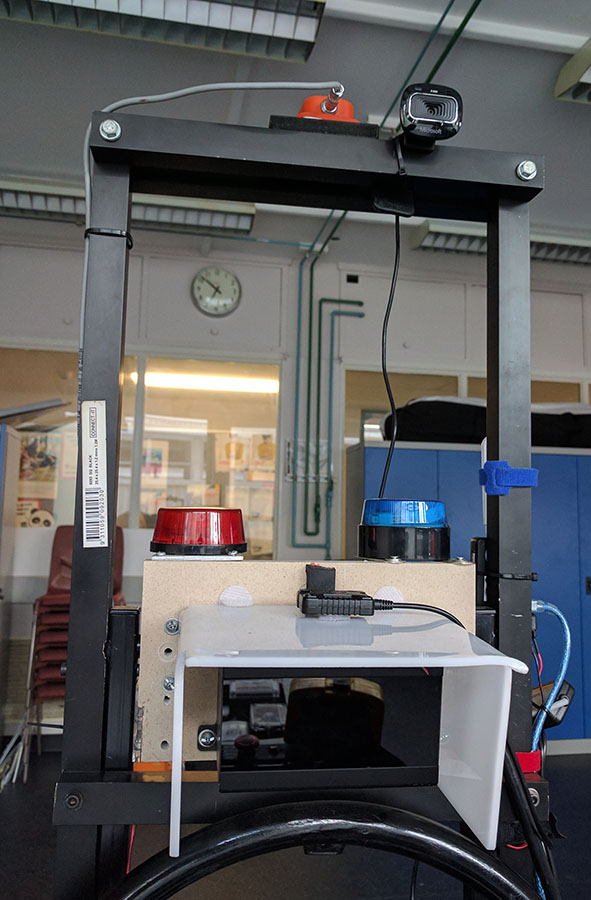
\includegraphics[width=0.35\linewidth]{cammount}
	\caption[Camera mounting location]{The camera is mounted above the LiDAR system from~\cite{drage_lidar_2015}, beside the IMU.}
	\label{fig:5:cam}
\end{figure}

\begin{table}[H]
	\caption{LiDAR Characteristics}
	\label{tablidar}
	\centering
	\begin{tabularx}{0.85\textwidth}{>{\raggedright}p{3cm} X}
		\toprule
		\bfseries Specification & \bfseries Value\\
		\midrule
		Technology & Time of flight (output of distance and echo pulse width)\\
		Range & 200 m\\
		Field of View (Horiz / Vert) & \ang{85} / \ang{3.2}\\
		Layers & 4\\
		Echo Detection & 3 measurements per pulse\\
		Update Rate & Up to 50Hz\\
		Accuracy & 10cm\\
		\bottomrule
	\end{tabularx}
\end{table}

The following subsections describe the process of achieving visual autonomous driving for our project using semantic segmentation with respect to its application environment and its driving sequences.

\subsection{Application Environment}
SegNet was tested within the grounds of the University of Western Australia (UWA), which is the same location that the LiDAR system was tested in~\cite{drage_lidar_2015}. The roads within UWA offers a similar drive environment to standard suburban roads. These single carriageway roads are of low traffic density, with views of pedestrians, faculty buildings, and vegetation for SegNet to recognise and segment. As a feasibility test, we also tested SegNet off a car-mounted dashcam recording while driving on local roads. 

This application environment was selected to test the suitability of using SegNet for autonomous driving locally and to gauge the visual autonomous navigation performance of the vehicle. To achieve a successful autonomous drive using SegNet on the vehicle, road edges and lane markings must be properly recognised, before the application can be subsequently expanded onto a road-licensed vehicle.

It should be noted that our initial implementation uses the trained dataset from the University of Cambridge, CamVid~\cite{badrinarayanan_segnet:_2017}. This dataset was recorded in the City of Cambridge, England. Like most British cities, Cambridge's roads are often narrow, with dense buildings by the side. There is also a large pedestrian population due to it being an academic city. Comparatively, roads in Perth are generally wider, with a sparser build-up density than Cambridge. Its low population density means that there are fewer road pedestrians as compared to Cambridge. The ground terrain around Perth is mostly flat, with long sunshine hours. This means that one can generally expect excellent road visibility on Western Australian roads on most days. However, during poor visibility and night time drives, suburban roads around Perth are generally poorly lit, which may affect road segmentation accuracy. By testing this dataset, we will subsequently contemplate on the need to record and use a dataset from Perth for more accurate segmentation results.

\subsection{Autonomous Driving Procedures}
To use SegNet's output for autonomous driving, we assume that the car begins with a position in the middle of the road lane and that the road incline is flat. By mounting the camera at a fixed position on the car, the central driving position of the car can be obtained, along with distance measurements from the road edges to the left and right sides of the car. With the camera, this is done by identifying and segregating a fixed trapezoidal image region that encapsulates the road segment, which is then transformed into a birds-eye view perspective to obtain vehicle's position with respect to the road's centre. By scaling the road width according to the Australian standards of 3.3--3.5 m, along with the detected road edges and/or lane markings on SegNet's output, the distance from the vehicle's centre to the left and right road edges/lanes can is obtained as Fig~\ref{fig:5:4pane}, with its confidence value determined by the successful detection of road edges or lane markings. From these three sections distance thresholds for the left and right edges or lane markers distances for the car to autonomously centre itself on the road while driving. We call this road centring. In the event where lane markers are not found, road edges will be used instead.

To perform road centring, the car must steer itself in the opposite direction when it crosses the distance threshold to either the left or right road edge/lane markers. The distance from the car to the road edges or lane markers are constantly analysed. If the car is too close to the edge or lane marker, the road centring algorithm will then send commands to the drive system to steer away from the edges with fine adjustments, until the car is cleared from the distance threshold.

\begin{figure}[H]
	\centering
	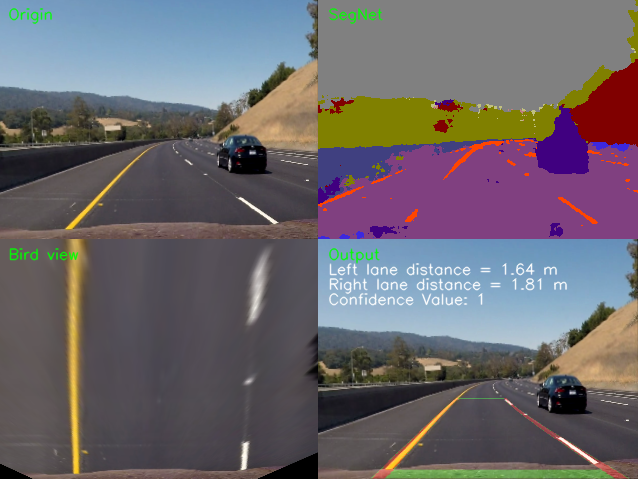
\includegraphics[width=0.8\linewidth]{4pane}
	\caption[Lane distance measurements with SegNet]{Lane distance measurements with SegNet's output on Udacity's Self-Driving Car Nanodegree recording~\cite{udacity_self-driving_2017} as the input in ``Origin''.}
	\label{fig:5:4pane}
\end{figure}

\section{Testing and Evaluations}
\subsection{Methodology} \label{secmethod}
Testing begins with the calibration of the camera, where distance measurements in the real world will be represented in pixel ratios on SegNet's output. Here, we calibrated a Microsoft LifeCam HD-3000 camera. This was done by measuring the distances between road bollards in front of the parked vehicle on the road as illustrated in Fig.~\ref{fig:5:front}.

\begin{figure}[H]
	\centering
	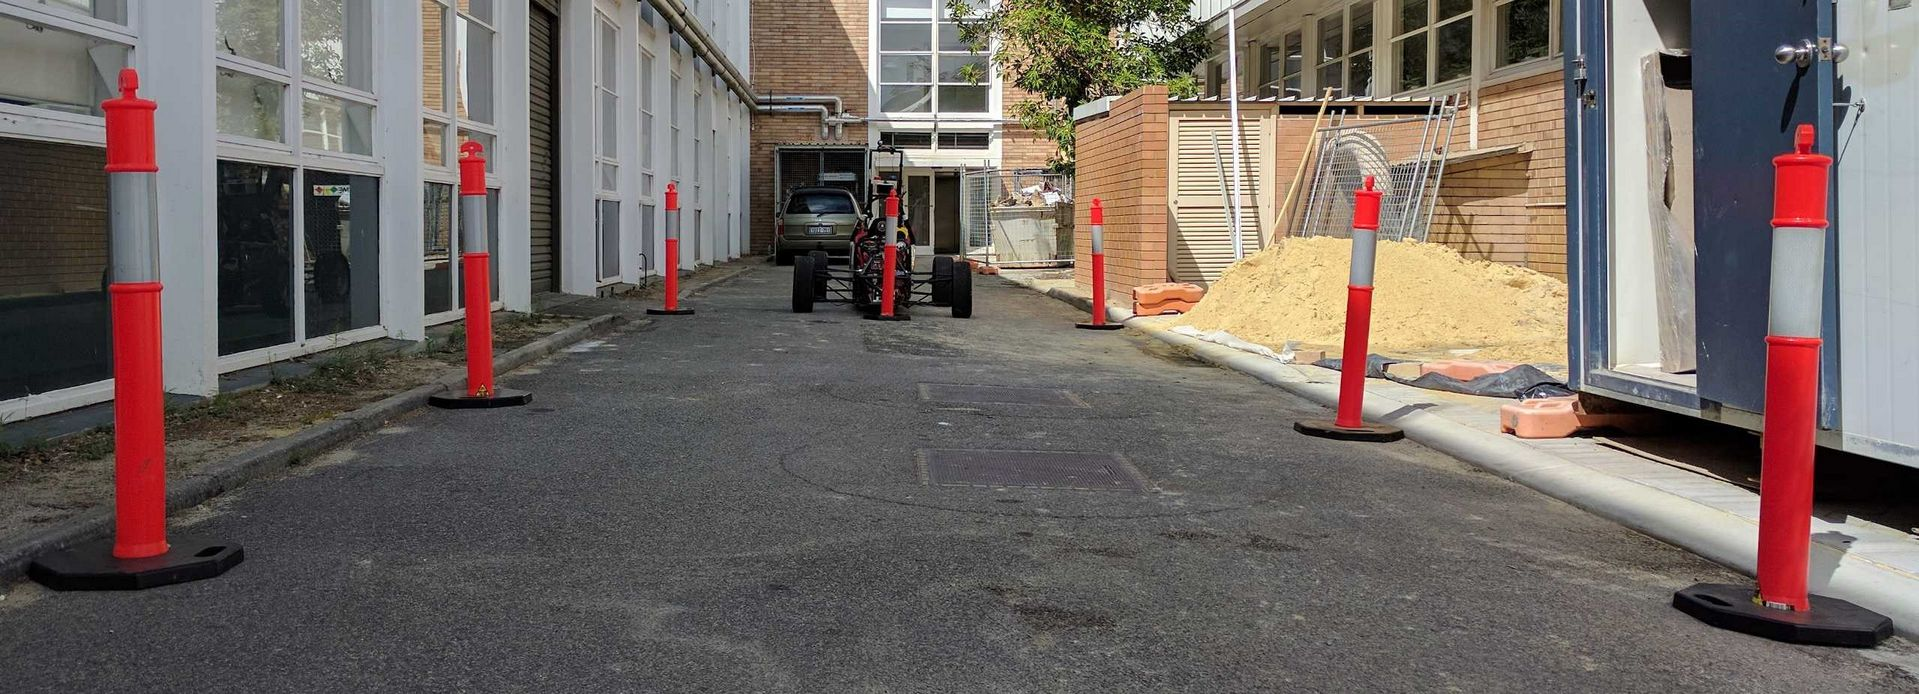
\includegraphics[width=0.8\linewidth]{front}
	\caption[Bollards' position with reference to the car]{Photo illustrating the bollards' position with reference to the car in the centre.}
	\label{fig:5:front}
\end{figure}

The bollards are placed a three-row formation to allow distance measurements from two-point distances on the frame. The first row of bollards on the car establishes the starting distance, with the centre bollard measuring the distance from the camera to the front of the car, while ensuring that the camera is pointed to the centre of the car. All distances are measured from the base at the centre of each bollard. Subsequently, a topological representation of the measurements can be illustrated in Fig.~\ref{fig:5:distances}, which is then represented again in the camera frame in Fig.~\ref{fig:5:bollards}. These measurements are verified with the LiDAR plot at that position as illustrated in Fig.~\ref{fig:5:lidarb}, where the bollards (represented as dot plots) are clearly present around the 2 m, 8 m and 10 m mark on the y-axis. From Fig.~\ref{fig:5:bollards}, each image pixel was calculated to represent 17 mm and 23 mm when measured from 8.5 m and 11.6 m respectively from the camera, and that a level road will converge at around \ang{41} on the camera frame.

The LiDAR readings complement SegNet's output for road edge detection, whereby we use our Kalman Filtered Linear Regression Model as described in~\cite{drage_lidar_2015}. Our algorithm minimises the square residuals between the fit line $y$ and the data ($x_i$, $y_i$), where the most suitable data line will be obtained for a given data set, and its success measured by the product-moment correlation coefficient $r$. The slope $b$ and $r$ values are given as~\eqref{eqn:5:1}.
\begin{subequations}
	\label{eqn:5:1}
	\begin{align}
		y &= (\bar{y}-b\bar{x})+bx \\
		r &= \frac{s_{xy}}{s_x s_y}%x = \sum\limits_{i=0}^{z} 2^{i}Q
	\end{align}
\end{subequations}
where:
\begin{subequations}
	\label{eqn:5:2}
	\begin{align}
	b &= \frac{s_{xy}}{s_x}^2\\
	s_{xy} &= \frac{\sum_{i=1}^{n} x_i y_i}{n}-\bar{x}\bar{y} \\
	{s_x}^2 &= \frac{\sum_{i=1}^{n} {x_i}^2}{n}-\bar{x}^2 \\
	{s_y}^2 &= \frac{\sum_{i=1}^{n} {y_i}^2}{n}-\bar{y}^2
	\end{align}
\end{subequations}

\nomenclature[a-x]{$x$}{$x$-coordinate (Cartesian system)} 
\nomenclature[a-y]{$y$}{$y$-coordinate (Cartesian system)} 
\nomenclature[a-r]{$r$}{Product-moment correlation [Chapter~\ref{ch:semseg}]} 
\nomenclature[a-b]{$b$}{Slope} 

\begin{figure}[H]
	\centering
	\def\svgwidth{0.4\linewidth}
	\input{Chapter5/Figs/PDF/distances.pdf_tex}
	\caption[Topological distance between bollards and car camera]{The topological distance between bollards (dots) and the camera on the car (shaded square).}
	\label{fig:5:distances}
\end{figure}

\begin{figure}[H]
	\centering
	\def\svgwidth{0.6\linewidth}
	\input{Chapter5/Figs/PDF/bollards.pdf_tex}
	\caption{Frame captured from the vehicle's camera for distance calibration.}
	\label{fig:5:bollards}
\end{figure}

\begin{figure}[H]
	\centering
	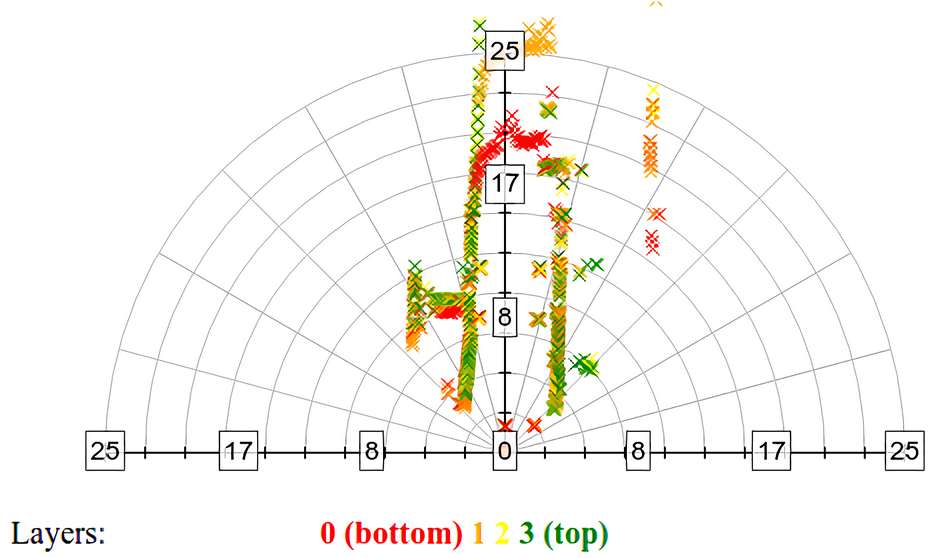
\includegraphics[width=0.8\linewidth]{bollardslidar}
	\caption[Calibration LiDAR plot]{LiDAR plot showing the detected road edges and the bollards' positions from the car where Fig.~\ref{fig:5:bollards} was captured. The graph axes measure distances in metres.}
	\label{fig:5:lidarb}
\end{figure}

With a calibrated camera and LiDAR, the SAE car was driven around the application environment while the camera is recording. The recorded camera footage was used as an input for SegNet. For testing purposes, these footages were processed off-line with SegNet running off an Nvidia GTX Titan X GPU with a 480 by 360-pixel resolution, which resulted in a segmented image output at a consistent 10 frames per second (FPS) sampled at each video frame. This framerate is consistent with the visual autonomous driving results published by Nvidia in~\cite{bojarski_end_2016}, making it adequate for autonomous driving. Further work is required for real-time on-line processing on the Jetson TX1. Likewise, LiDAR plots are also recorded during the duration of the drive, where timestamps are used to synchronise outputs.

\nomenclature[z-fps]{FPS}{Frames per second}

\subsection{Results and Discussions}
Results from semantic segmentation are presented first on open roads with a dash cam recording, and then on the UWA campus ground with the SAE car. Image results in this section are presented with the left image showing segmentation input, and the right image showing its output through SegNet. In the case of false detections, they will be measured in their pixel accuracy (PA). This is done by finding the percentages of road regions, which is done by counting the number of falsely detected pixels $p_{ii}$ against the total number of pixels $k$ in the road region $p_{ij}$ for that image frame:

\begin{align}
\mathrm{PA} = \frac{\sum_{i=0}^k p_{ii}}{\sum_{i=0}^k \sum_{j=0}^k p_{ij}}
\end{align}

\nomenclature[z-pa]{PA}{Pixel accuracy}
\nomenclature[a-p]{$p$}{Classified pixel} 

Segmentation results from the open road testing from the dashcam footage yielded consistently favourable results, as shown in Fig.~\ref{fig:5:road}. Recordings were captured on a clear day, driving on a low traffic dual carriageway. The road region is accurately segmented with negligible false detections. In addition to the road and its markings, SegNet can detect and segment the speed limit sign and the right turn sign ahead. All vehicles and vegetation were also properly detected and segmented. The minor false detections in the sky region are due to the CamVid dataset being trained on a cloudy day, but this should not affect road detection accuracy in any way. This result confirms the feasibility that a CamVid-trained SegNet can be implemented for autonomous driving in the Perth metro area.

\begin{figure}[H]
	\centering
	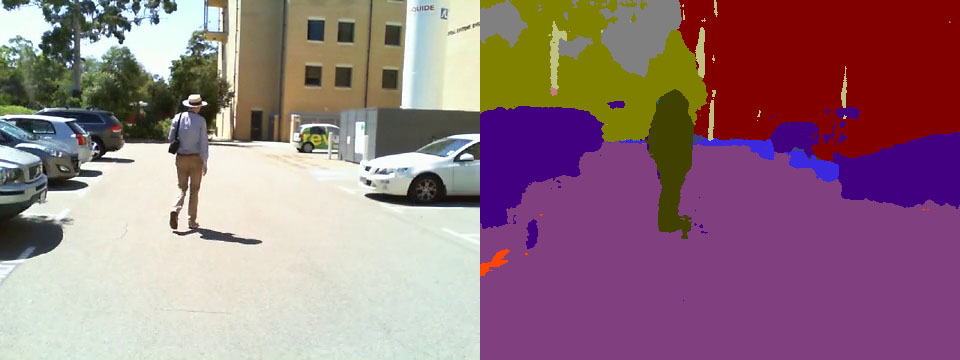
\includegraphics[width=0.8\linewidth]{segnet}
	\caption[SegNet results on a Perth dual carriageway]{SegNet's input (left) and output (right) for a dual carriageway in the Perth metro area.}
	\label{fig:5:road}
\end{figure}

Tests were subsequently performed on the SAE car for a vision-LiDAR-based implementation. Here, runs on campus grounds were recorded using the camera while manually driven on the SAE car following a predetermined route on campus. The car traversed across roads and pavements and the segmentation results are as follows.

\begin{figure}[H]
	\centering
	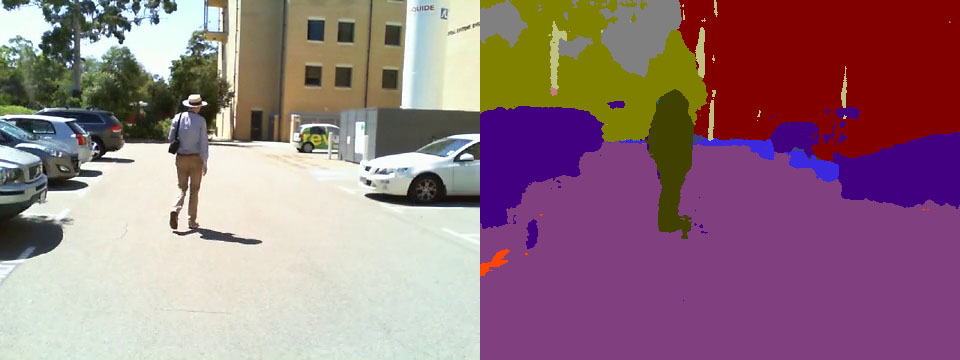
\includegraphics[width=0.8\linewidth]{2}
	\caption{Segmentation results from a parking area on campus grounds.}
	\label{fig:5:carpark}
\end{figure}

\begin{figure}[H]
	\centering
	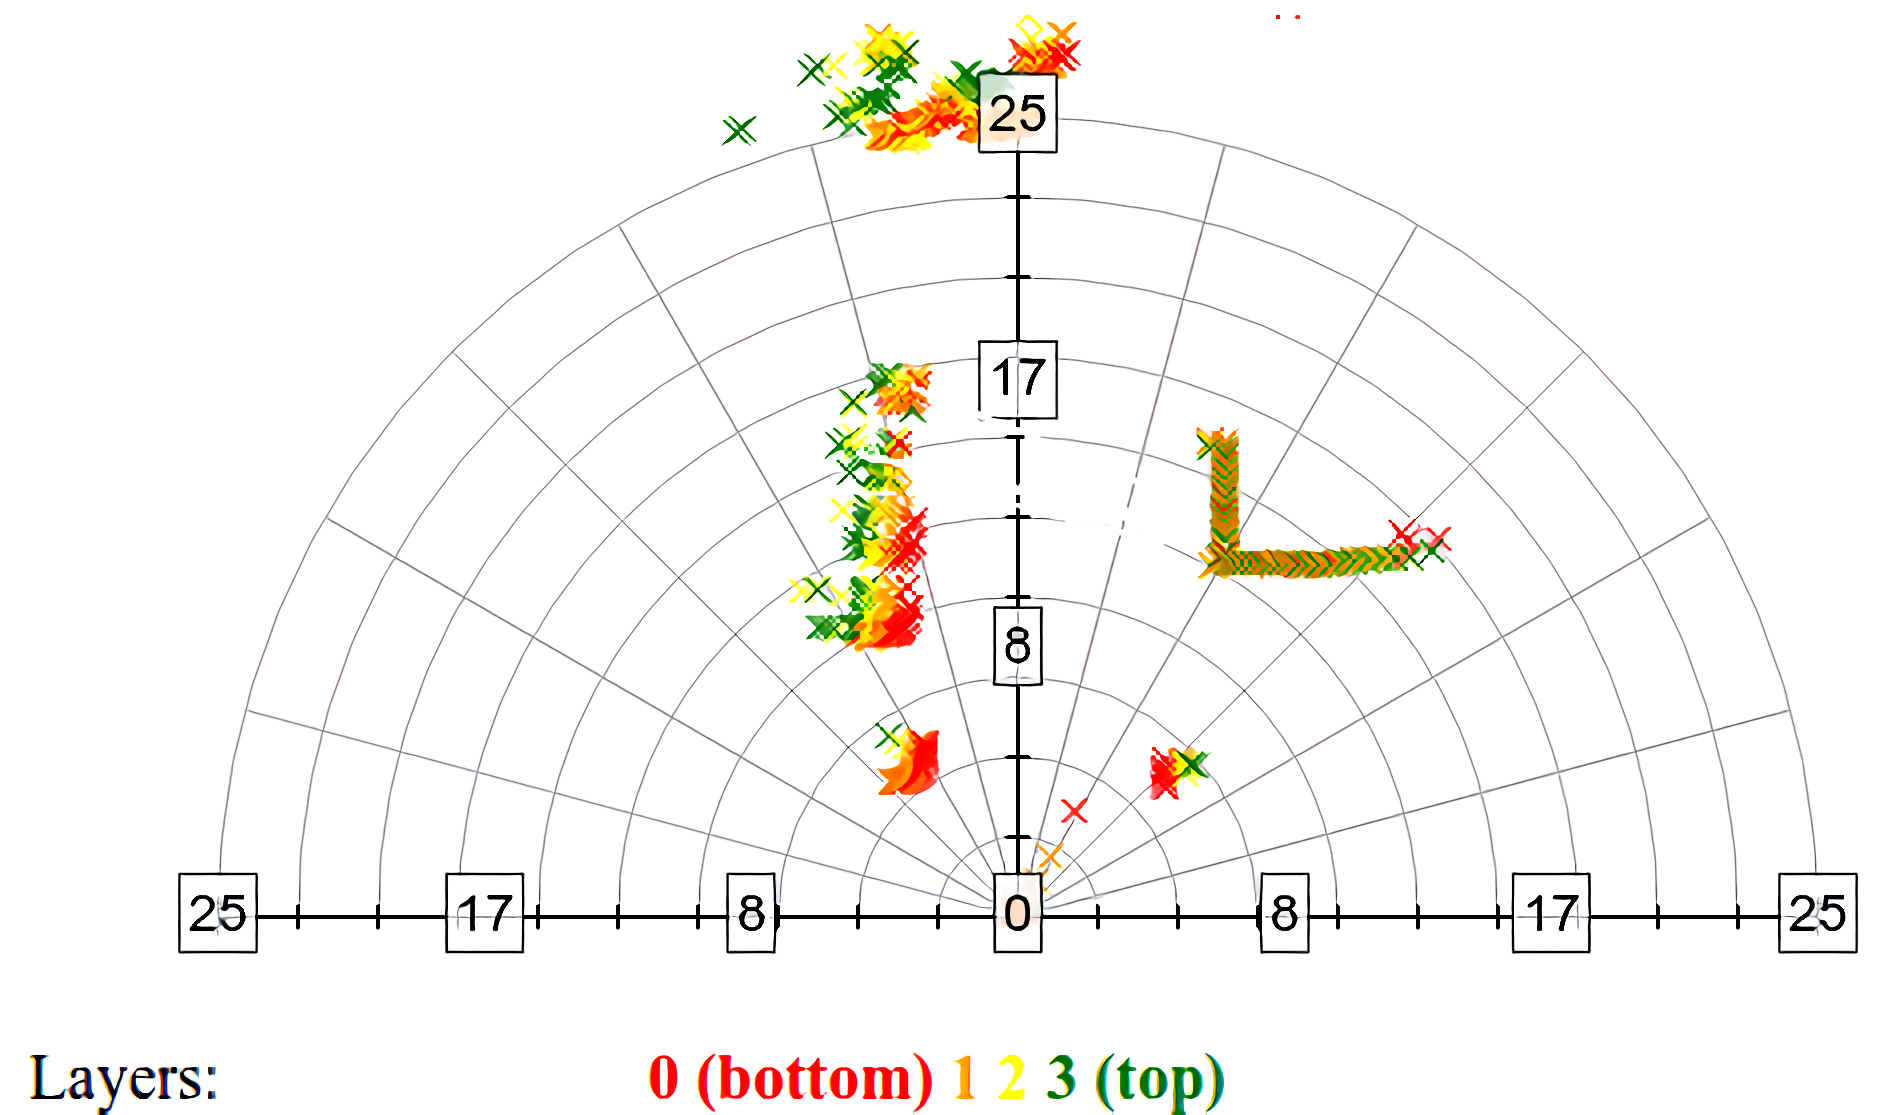
\includegraphics[width=0.8\linewidth]{luxplot}
	\caption[LiDAR plot at the position of Fig.~\ref{fig:5:carpark}]{LiDAR plot showing the detected parked vehicles at the position where Fig.~\ref{fig:5:carpark} was captured. The graph axes measure distances in metres.}
	\label{fig:5:lidar}
\end{figure}

\begin{figure}[H]
	\centering
	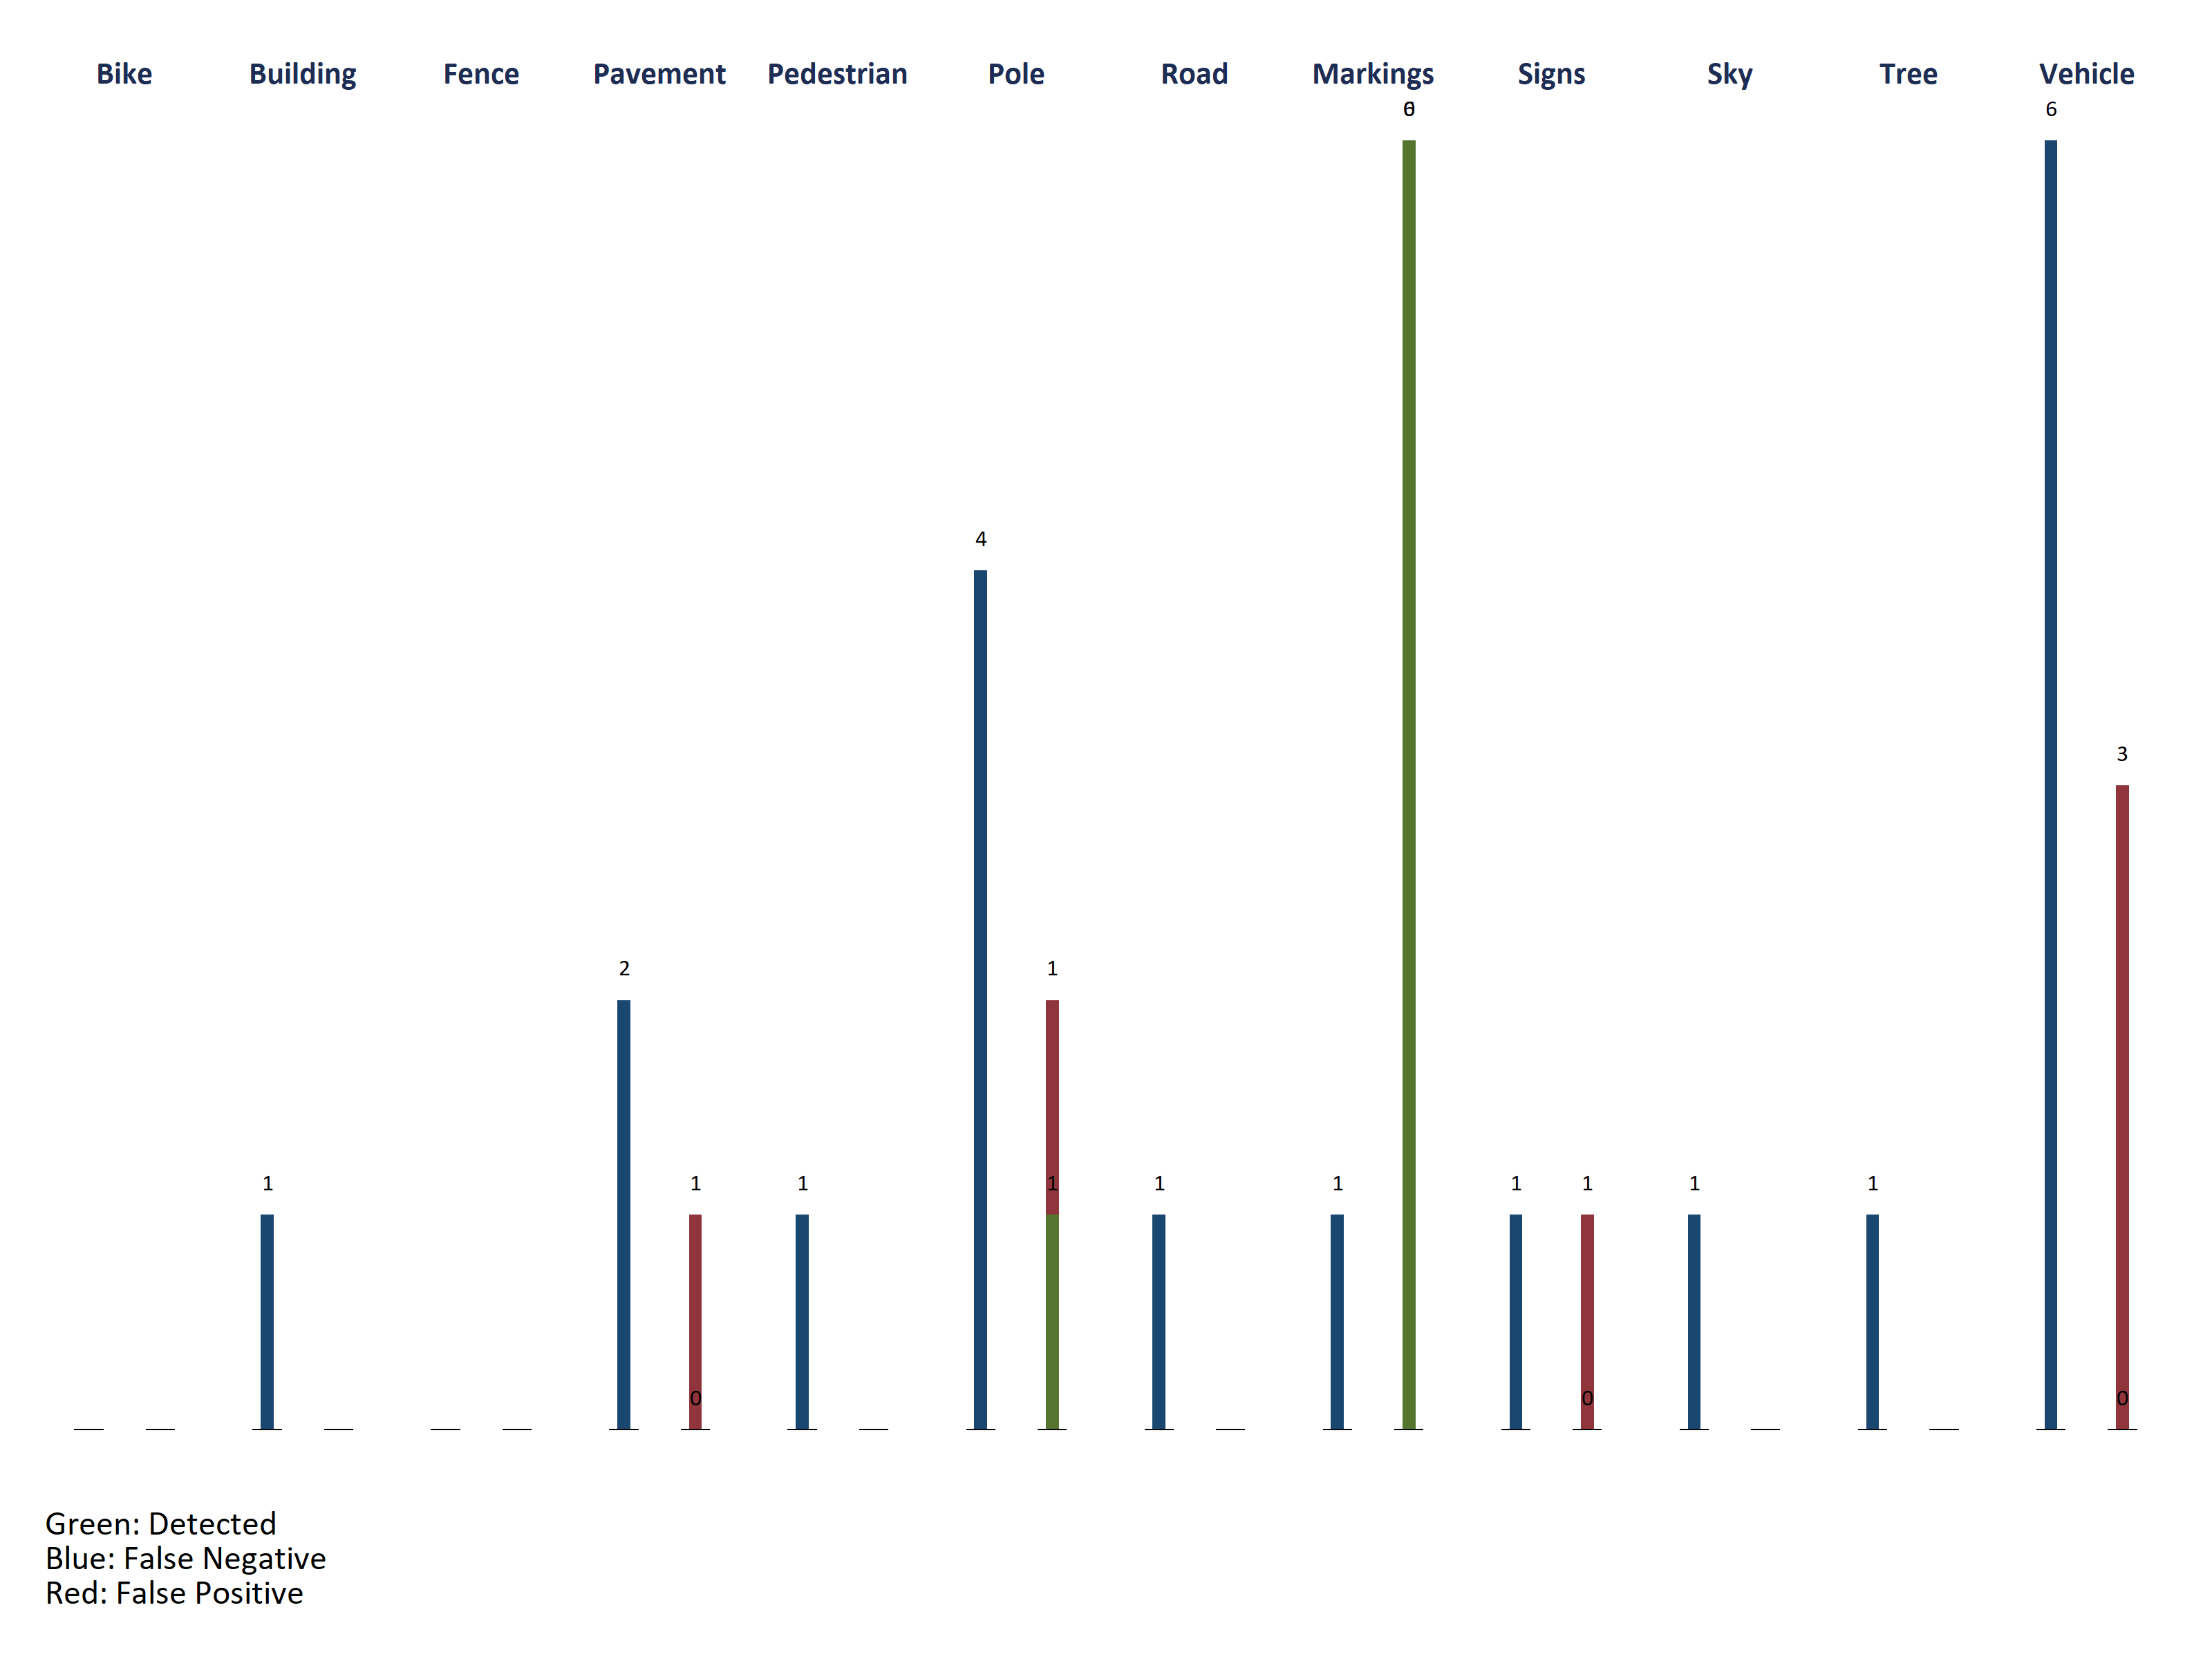
\includegraphics[width=0.9\linewidth]{figure_2}
	\caption[Detected objects and their errors]{The number of detected objects along their errors in detections according to the objects.}
	\label{fig:5:graph}
\end{figure}

The test run began with a drive through the car park. SegNet's output in Fig.~\ref{fig:5:carpark} shows that the image was segmented with good accuracy. With the exception of some minor (0.69\%)  false detections on the car's shadows on the left side, the road, parking lane, and pavements were properly segmented, along with the pedestrian and vehicles. With the LiDAR actively measuring the distance from the parked vehicles to the SAE car (see Fig.~\ref{fig:5:lidar}). Here, we adopt the Linear Regression model that we described in Section~\ref{secmethod}, which plots the road edge position from the parked vehicles so that a fixed distance can be kept between the autonomous cars and the parked vehicles. We have also counted the number of detected objects along with their positive and negative false detections, which are plotted according to their detection/error pairs in Fig.~\ref{fig:5:graph}, whereby the labelled number on each bar indicated the number of correctly identified objects, if present. 

\begin{figure}[H]
	\centering
	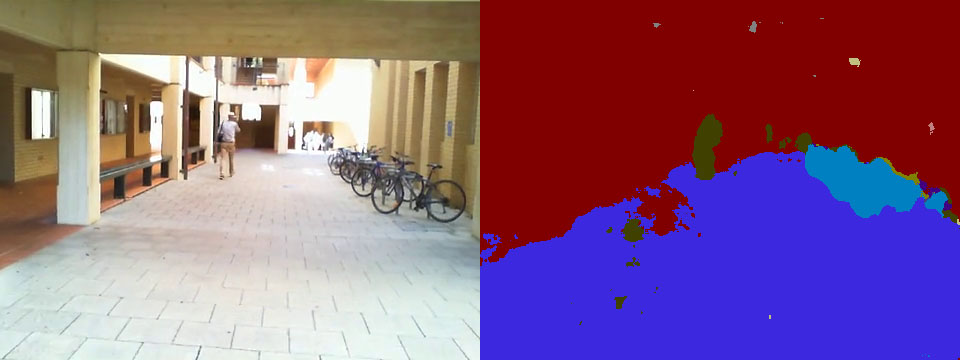
\includegraphics[width=0.8\linewidth]{3}
	\caption{Segmentation results on pavement between faculty buildings.}
	\label{fig:5:pavement}
\end{figure}

From the parking area, the car drives onto the pavement between faculty buildings. From Fig.~\ref{fig:5:pavement}, SegNet could discern pavements from roads as the grounds are now coloured blue. In addition, it was also able to detect the bicycles parked towards the right, and the pedestrians in the distance. False detections are present on the left side of the pavement, where it is incorrectly detected as buildings and pedestrians due to uneven lighting, accounting for 2.83\% of the total pavement region. 

\begin{figure}[H]
	\centering
	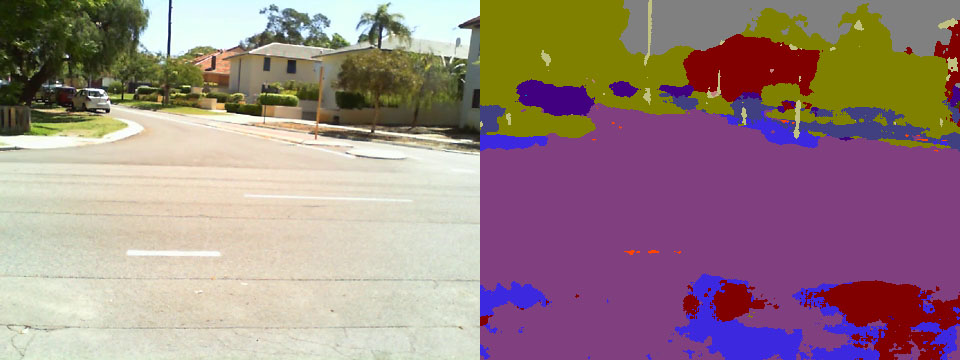
\includegraphics[width=0.8\linewidth]{4}
	\caption{Segmentation results at a road junction.}
	\label{fig:5:junction}
\end{figure}

Fig.~\ref{fig:5:junction} was captured when the car was stopping at a suburban road junction beside the campus. The segmentation output from this figure shows that while the objects in the distance were properly segmented, some parts at the bottom of the image was incorrectly classified as pavements and buildings, which makes up 16.19\% of the road region. This was partly due to the clear weather resulting in a high brightness recording, while SegNet was expecting a darker surface to classify roads. 

\begin{figure}[H]
	\centering
	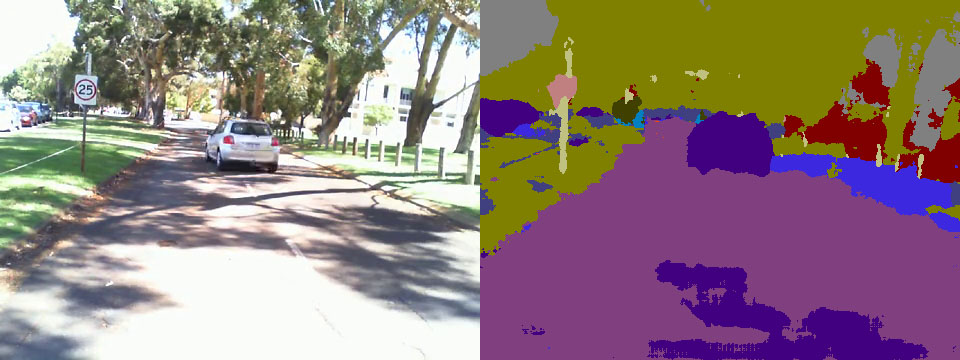
\includegraphics[width=0.8\linewidth]{5}
	\caption{Segmentation results on a road with pronounced shadows.}
	\label{fig:5:shadows}
\end{figure}

Fig.~\ref{fig:5:shadows} was captured while the car was driving on a shadowed road on campus. The shadows on the road introduced a high contrast region, and that the bottom portion of the road was overexposed, resulting in a false classification of 13.93\% and undetected lane markers. However, the overtaking vehicle, vegetation, road sign, and building were correctly segmented. When presented with a false detection on the road as with Figure~\ref{fig:5:road}, results from the LiDAR road edge detection system will compensate the regions of false detection, as the road and road edges were properly measured by the LiDAR system. 

\begin{table}[H]
	\renewcommand{\arraystretch}{1.3}
	\caption[Semantic segmentation accuracy]{The number of road region pixels and its false detections pixels in that region for each figure along with their error percentages. }
	\label{tabpixelcount}
	\centering
	\begin{tabular}{crrr}
		\toprule
		        Fig.         & Road Pixels & False Classifications &   Error \\ \midrule
		 ~\ref{fig:5:road}   &       41648 &                    16 &  0.04\% \\
		\ref{fig:5:carpark}  &       86561 &                   600 &  0.69\% \\
		\ref{fig:5:pavement} &       76731 &                  2168 &  2.83\% \\
		\ref{fig:5:junction} &      108684 &                 17595 & 16.19\% \\
		\ref{fig:5:shadows}  &       83831 &                 11679 & 13.93\% \\ \bottomrule
	\end{tabular}
\end{table}

The false detection rates for each of the example figures is summarised as Table~\ref{tabpixelcount}, which also tabulates the number of road pixels in each detected road segments for each figure, along with the number of falsely classified pixels within that road segment. From these numbers, the detection error is calculated as a percentage that corresponds to the area of each figure's road segments. The false detection rate is at its highest in Fig.~\ref{fig:5:junction}, where the road region encompasses most of the frame, the unevenness in road surface and lighting is the main contributor to this error rate. Conversely, Fig.~\ref{fig:5:road} records the lowest false detection rate its road segment, as the road area was well-defined, and the frame was properly exposed. 

\section{Conclusion}
We have presented a semantic segmentation-based visual navigation approach for autonomous ground vehicles. This approach improves on existing LiDAR-based vehicles to introduce object recognition and classification while driving. SegNet adequately performs semantic segmentation to recognise roads and lane markers, which in turn allows the vehicle to maintain a safe distance from the road and lane edges in addition to LiDAR measurements. We have also shown that the segmentation results from SegNet on the CamVid dataset is satisfactory on Perth metro roads. With a calibrated camera, visual autonomous driving can be achieved using real-time semantic segmentation. Future works will focus on the complete on-line implementation of SegNet on the SAE car for real-time visual autonomous driving.